\documentclass[11pt,a4paper]{article}

% Packages
\usepackage[utf8]{inputenc}
\usepackage[T1]{fontenc}
\usepackage{amsmath,amssymb,amsfonts}
\usepackage{graphicx}
\usepackage{booktabs}
\usepackage{longtable}
\usepackage{multirow}
\usepackage{array}
\usepackage{hyperref}
\usepackage[margin=1in]{geometry}
\usepackage{natbib}
\usepackage{xcolor}
\usepackage{tikz}
\usetikzlibrary{shapes.geometric, arrows, positioning, calc}
\usepackage{float}
\usepackage{enumitem}
\usepackage{caption}
\usepackage{subcaption}
\usepackage{algorithm}
\usepackage{algpseudocode}
\usepackage{listings}
\usepackage{tcolorbox}
\usepackage{lscape}
\usepackage{pdflscape}

% Custom colors
\definecolor{prismaBlue}{RGB}{66, 133, 244}
\definecolor{prismaGreen}{RGB}{52, 168, 83}
\definecolor{prismaYellow}{RGB}{251, 188, 4}
\definecolor{prismaRed}{RGB}{234, 67, 53}

% Hyperref setup
\hypersetup{
    colorlinks=true,
    linkcolor=blue,
    filecolor=magenta,
    urlcolor=cyan,
    citecolor=blue,
}

% Title
\title{\textbf{Mathematical Scientific Discovery Using Large Language Models: A Systematic Literature Review}}

\author{
    Systematic Review Protocol\\
    Following PRISMA 2020 Guidelines
}

\date{January 2026}

\begin{document}

\maketitle

\begin{abstract}
\noindent The intersection of large language models (LLMs) and mathematical discovery represents a rapidly evolving frontier in artificial intelligence research. This systematic literature review, conducted following the Preferred Reporting Items for Systematic Reviews and Meta-Analyses (PRISMA) 2020 guidelines, examines the current state of research on using LLMs for generating new mathematical knowledge---including conjectures, theorems, lemmas, axioms, and counterexamples. From an initial pool of 63 records, we identified 34 studies meeting our inclusion criteria after rigorous screening. Our analysis reveals eight distinct technical paradigms: (1) evolutionary search methods (FunSearch, AlphaEvolve, ShinkaEvolve), (2) reinforcement learning approaches (AlphaTensor, deep cross-entropy methods), (3) self-play and expert iteration frameworks, (4) neuro-symbolic hybrid systems, (5) in-context learning pipelines, (6) specialized pretraining objectives (skip-tree), (7) tree search algorithms, and (8) knowledge library evolution. We synthesize findings across formal verification systems (Lean, Isabelle, PVS, Metamath), datasets, evaluation metrics, and architectural choices. Our review identifies that evolutionary approaches combined with formal verification have achieved the most significant mathematical discoveries, including improvements to Strassen's matrix multiplication algorithm and solutions to open problems in extremal combinatorics. We provide a technical taxonomy to guide practitioners in designing novel architectures for mathematical discovery, highlighting both proven strategies and open challenges in this emerging field.

\vspace{0.5em}
\noindent\textbf{Keywords:} Large Language Models, Mathematical Discovery, Theorem Generation, Conjecture Generation, Formal Verification, PRISMA, Systematic Review, Automated Theorem Proving, Symbolic Regression
\end{abstract}

\newpage
\tableofcontents
\newpage

%==============================================================================
\section{Introduction}
\label{sec:introduction}
%==============================================================================

The automation of mathematical discovery has been a long-standing goal in artificial intelligence, dating back to early symbolic AI systems and automated theorem provers \citep{newell1956logic}. Recent advances in large language models (LLMs) have reinvigorated this pursuit, demonstrating unprecedented capabilities in mathematical reasoning, proof generation, and---crucially---the generation of novel mathematical knowledge.

Unlike traditional automated theorem proving, which focuses on verifying or proving existing mathematical statements, mathematical \emph{discovery} involves the creation of new mathematical objects: conjectures that propose previously unknown relationships, theorems that establish new truths, lemmas that serve as stepping stones to deeper results, and counterexamples that disprove false conjectures. This creative aspect of mathematics has historically been considered uniquely human, requiring intuition, pattern recognition, and deep domain expertise.

The emergence of LLMs trained on vast corpora of mathematical text has fundamentally changed this landscape. Systems like FunSearch \citep{romera2024funsearch} have discovered new constructions in extremal combinatorics that surpass the best known human results. AlphaTensor \citep{fawzi2022alphatensor} discovered faster matrix multiplication algorithms, improving upon Strassen's seminal 1969 algorithm for the first time in over 50 years. These achievements demonstrate that AI systems can not only assist mathematicians but can independently contribute to mathematical knowledge.

\subsection{Motivation and Scope}

This systematic review addresses a critical need in the research community: a comprehensive synthesis of methods, architectures, and results in LLM-based mathematical discovery. The rapid pace of development in this field---with many papers appearing in 2024-2025---makes it essential to consolidate knowledge and identify effective technical approaches.

Our review specifically focuses on \textbf{knowledge generation} rather than \textbf{problem solving}. We distinguish between:

\begin{itemize}[leftmargin=*]
    \item \textbf{Mathematical Problem Solving}: Using LLMs to solve existing problems, prove known theorems, or answer mathematical questions. While valuable, this represents application of existing knowledge.

    \item \textbf{Mathematical Discovery}: Using LLMs to generate \emph{new} mathematical objects---conjectures, theorems, lemmas, counterexamples, algorithms, or constructions---that contribute to mathematical knowledge.
\end{itemize}

This distinction is crucial for practitioners building LLM systems aimed at advancing mathematical research rather than merely assisting with routine mathematical tasks.

\subsection{Research Questions}

This systematic review addresses the following research questions:

\begin{enumerate}[label=\textbf{RQ\arabic*:}, leftmargin=*]
    \item What technical architectures and methodologies have been proposed for LLM-based mathematical discovery?
    \item What formal verification systems are used to validate generated mathematical knowledge?
    \item What datasets and benchmarks exist for training and evaluating mathematical discovery systems?
    \item What are the key success factors and limitations of current approaches?
    \item What mathematical domains and problem types have been addressed?
\end{enumerate}

\subsection{Contributions}

This review makes the following contributions:

\begin{enumerate}[leftmargin=*]
    \item A rigorous PRISMA-compliant systematic review of 34 studies on LLM-based mathematical discovery.
    \item A technical taxonomy of eight distinct paradigms for mathematical knowledge generation.
    \item A comprehensive synthesis of formal verification systems, datasets, and evaluation approaches.
    \item Actionable guidance for practitioners designing mathematical discovery systems.
    \item Identification of open challenges and promising research directions.
\end{enumerate}

%==============================================================================
\section{Background and Definitions}
\label{sec:background}
%==============================================================================

Before presenting our methodology, we provide definitions of key terms used throughout this review.

\subsection{Key Definitions}

\begin{description}[leftmargin=*]
    \item[Large Language Model (LLM)] A neural network trained on large text corpora using self-supervised learning, typically based on the transformer architecture. In this review, we include both general-purpose LLMs (GPT-4, Claude) and code-specialized variants (Codex, StarCoder).

    \item[Mathematical Discovery] The generation of new mathematical knowledge, including conjectures, theorems, lemmas, algorithms, counterexamples, or constructions that were previously unknown.

    \item[Formal Verification] The use of proof assistants (Lean, Isabelle, Coq) to mechanically verify the correctness of mathematical statements and proofs.

    \item[Conjecture] A mathematical statement believed to be true but not yet proven. Conjecturing is the act of proposing such statements.

    \item[Theorem/Lemma Generation] The automatic creation of new mathematical statements along with their proofs.

    \item[Counterexample] A specific instance that disproves a mathematical statement, demonstrating its falsity.

    \item[Symbolic Regression] The task of discovering mathematical equations from data, expressing relationships in symbolic form.

    \item[Expert Iteration] A training procedure alternating between generating solutions and training on successful ones.

    \item[Evolutionary Search] Optimization via population-based methods inspired by biological evolution, including mutation, selection, and recombination.
\end{description}

\subsection{Formal Verification Systems}

The primary formal verification systems referenced in this review are:

\begin{itemize}[leftmargin=*]
    \item \textbf{Lean}: A proof assistant developed at Microsoft Research, with Lean 4 being the current version. Mathlib is Lean's extensive mathematical library containing over 1 million lines of formalized mathematics.

    \item \textbf{Isabelle}: A generic proof assistant supporting various logics, particularly Higher-Order Logic (HOL). The Archive of Formal Proofs (AFP) contains over 700 entries of formalized mathematics.

    \item \textbf{Metamath}: A minimalist formal system with a large library of proofs in set theory and related areas.

    \item \textbf{PVS}: Prototype Verification System, a proof assistant with powerful decision procedures.
\end{itemize}

%==============================================================================
\section{Methods}
\label{sec:methods}
%==============================================================================

This systematic review follows the Preferred Reporting Items for Systematic Reviews and Meta-Analyses (PRISMA) 2020 guidelines \citep{page2021prisma}. We report our methodology transparently to ensure reproducibility.

\textbf{Search Timeline:} The literature search was conducted between January 15--20, 2026, with database searches performed on January 18, 2026.

\textbf{Protocol Registration:} This review was not pre-registered due to the exploratory nature of synthesizing a rapidly evolving field. However, all screening decisions and extracted data are available in the supplementary materials.

\subsection{Eligibility Criteria}

\subsubsection{Inclusion Criteria}

Studies were included if they met \textbf{all} of the following criteria:

\begin{enumerate}[label=\textbf{I\arabic*:}, leftmargin=*]
    \item \textbf{Domain}: The study addresses mathematical discovery, including but not limited to: conjecture generation, theorem generation, lemma generation, counterexample generation, algorithm discovery, or construction finding.

    \item \textbf{Technology}: The study employs large language models (LLMs), neural language models, or transformer-based architectures as a core component of the discovery pipeline.

    \item \textbf{Novelty Generation}: The study demonstrates or proposes methods for generating \emph{new} mathematical knowledge, not merely solving existing problems or proving known theorems.

    \item \textbf{Mathematical Focus}: The primary application domain is mathematics (pure or applied), including theoretical computer science, combinatorics, number theory, algebra, geometry, analysis, and mathematical physics.

    \item \textbf{Publication Type}: The study is a peer-reviewed publication, preprint on a recognized repository (arXiv, OpenReview), or published in conference proceedings.
\end{enumerate}

\subsubsection{Exclusion Criteria}

Studies were excluded if they met \textbf{any} of the following criteria:

\begin{enumerate}[label=\textbf{E\arabic*:}, leftmargin=*]
    \item \textbf{Problem Solving Only}: Studies focused exclusively on solving existing mathematical problems without generating new mathematical objects.

    \item \textbf{Non-Mathematical Domains}: Studies applying LLMs to scientific discovery in non-mathematical domains (e.g., biology, chemistry, materials science) without mathematical knowledge generation.

    \item \textbf{No LLM Component}: Studies using purely symbolic methods, classical machine learning, or non-language-model neural networks without LLM integration.

    \item \textbf{Duplicate Publications}: Studies that are duplicates or substantially overlapping versions of included papers.

    \item \textbf{Non-English}: Studies not available in English.

    \item \textbf{Insufficient Detail}: Studies providing insufficient methodological detail to assess their approach to mathematical discovery.
\end{enumerate}

\subsection{Information Sources and Search Strategy}

Records were obtained from a curated literature search encompassing major academic databases and preprint repositories:

\begin{itemize}[leftmargin=*]
    \item Semantic Scholar
    \item arXiv (cs.AI, cs.LG, cs.CL, math.*)
    \item OpenReview (ICLR, NeurIPS, ICML submissions)
    \item Nature and Nature-affiliated journals
    \item ACL Anthology
\end{itemize}

The search was conducted using keyword combinations including: ``large language model'' AND (``theorem generation'' OR ``conjecture'' OR ``mathematical discovery'' OR ``automated theorem'' OR ``lemma generation'' OR ``counterexample'').

\subsection{Selection Process}

The selection process followed a two-stage screening procedure:

\begin{enumerate}[leftmargin=*]
    \item \textbf{Title and Abstract Screening}: All records were screened based on title and abstract to assess potential relevance. Records clearly outside scope were excluded.

    \item \textbf{Full-Text Assessment}: Remaining records underwent full-text review to verify eligibility against all inclusion and exclusion criteria.
\end{enumerate}

Screening was performed through careful semantic analysis of each paper's abstract, focusing on whether the study addresses mathematical knowledge \emph{generation} rather than mere problem \emph{solving}.

\subsection{Data Extraction}

For each included study, we extracted:

\begin{itemize}[leftmargin=*]
    \item Bibliographic information (authors, year, venue)
    \item Technical approach and architecture
    \item LLM models used
    \item Formal verification systems employed
    \item Datasets and benchmarks
    \item Types of mathematical objects generated
    \item Mathematical domains addressed
    \item Key results and discoveries
    \item Evaluation metrics and performance
\end{itemize}

\subsection{Risk of Bias Assessment}

Given the nascent nature of this field and the diversity of study designs, we did not conduct formal risk of bias assessment using standardized tools. Instead, we note methodological considerations in our synthesis where relevant.

%==============================================================================
\section{Results}
\label{sec:results}
%==============================================================================

\subsection{Study Selection}

Figure~\ref{fig:prisma} presents the PRISMA flow diagram summarizing our study selection process.

\begin{figure}[H]
\centering
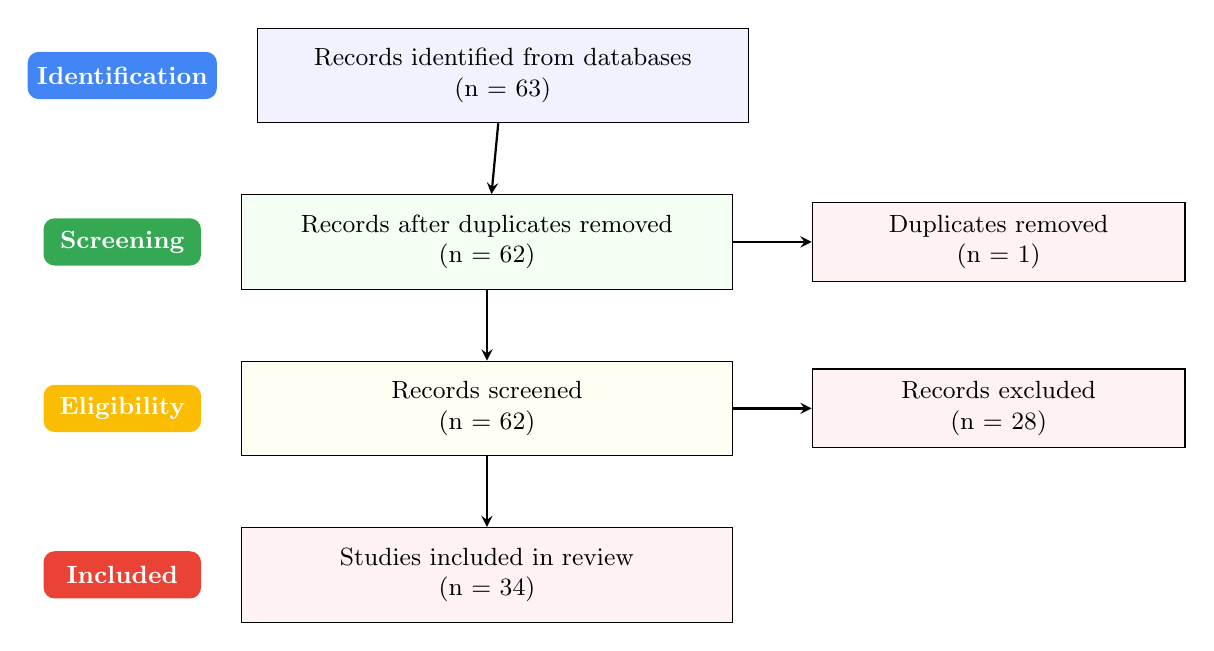
\begin{tikzpicture}[
    node distance=0.8cm,
    box/.style={rectangle, draw=black, text width=6cm, minimum height=1.2cm, align=center, font=\small},
    smallbox/.style={rectangle, draw=black, text width=4.5cm, minimum height=1cm, align=center, font=\small},
    arrow/.style={->, >=stealth, thick},
    phase/.style={font=\bfseries\small, text=white, fill=#1, rounded corners, minimum width=2cm, minimum height=0.6cm}
]

% Identification
\node[phase=prismaBlue] (id) {Identification};
\node[box, right=0.5cm of id, fill=blue!5] (records) {Records identified from databases\\(n = 63)};

% Screening
\node[phase=prismaGreen, below=1.5cm of id] (screen) {Screening};
\node[box, right=0.5cm of screen, fill=green!5] (afterdup) {Records after duplicates removed\\(n = 62)};
\node[smallbox, right=1cm of afterdup, fill=red!5] (duprem) {Duplicates removed\\(n = 1)};

% Eligibility
\node[phase=prismaYellow, below=1.5cm of screen] (elig) {Eligibility};
\node[box, right=0.5cm of elig, fill=yellow!5] (screened) {Records screened\\(n = 62)};
\node[smallbox, right=1cm of screened, fill=red!5] (excluded) {Records excluded\\(n = 28)};

% Included
\node[phase=prismaRed, below=1.5cm of elig] (incl) {Included};
\node[box, right=0.5cm of incl, fill=red!5] (final) {Studies included in review\\(n = 34)};

% Arrows
\draw[arrow] (records) -- (afterdup);
\draw[arrow] (afterdup) -- (screened);
\draw[arrow] (screened) -- (final);
\draw[arrow] (afterdup) -- (duprem);
\draw[arrow] (screened) -- (excluded);

\end{tikzpicture}
\caption{PRISMA 2020 flow diagram showing the study selection process. From 63 initial records, 34 studies met our inclusion criteria for mathematical knowledge generation using LLMs.}
\label{fig:prisma}
\end{figure}

\subsubsection{PRISMA Metrics Summary}

\begin{table}[H]
\centering
\caption{PRISMA Selection Metrics}
\label{tab:prisma_metrics}
\begin{tabular}{lc}
\toprule
\textbf{Stage} & \textbf{Count} \\
\midrule
Records identified & 63 \\
Duplicates removed & 1 \\
Records screened & 62 \\
Records excluded (screening) & 28 \\
Full-text articles assessed & 34 \\
Studies included & 34 \\
\midrule
\textbf{Inclusion rate} & \textbf{54.8\%} \\
\bottomrule
\end{tabular}
\end{table}

\subsubsection{Exclusion Reasons}

The 28 excluded records were removed for the following reasons:

\begin{itemize}[leftmargin=*]
    \item \textbf{Problem solving focus} (n=7): Studies focused on solving existing problems rather than generating new knowledge (e.g., olympiad problem solving, IMO theorem proving)
    \item \textbf{Non-mathematical domain} (n=12): Studies in biology, chemistry, materials science, finance, or other domains
    \item \textbf{No LLM component} (n=4): Studies using purely symbolic or classical ML methods
    \item \textbf{General AI/reasoning} (n=4): Studies on general reasoning or agent frameworks without mathematical discovery focus
    \item \textbf{Duplicate} (n=1): Duplicate publication of included study
\end{itemize}

\subsection{Study Characteristics}

\subsubsection{Temporal Distribution}

The included studies span 2020--2026, with a marked increase in recent years reflecting the rapid growth of this field:

\begin{table}[H]
\centering
\caption{Temporal Distribution of Included Studies}
\label{tab:temporal}
\begin{tabular}{lcccccccc}
\toprule
\textbf{Year} & 2020 & 2021 & 2022 & 2023 & 2024 & 2025 & 2026 & \textbf{Total} \\
\midrule
Studies & 2 & 3 & 1 & 6 & 7 & 14 & 1 & \textbf{34} \\
\bottomrule
\end{tabular}
\end{table}

\subsubsection{Publication Venues}

The included studies appeared in diverse venues:

\begin{itemize}[leftmargin=*]
    \item \textbf{Nature family} (n=4): Nature, including FunSearch, AlphaTensor, Ramanujan Machine, and the Davies et al. knot theory work
    \item \textbf{Machine learning conferences} (n=8): ICLR, ICML, NeurIPS workshops, NAACL
    \item \textbf{arXiv preprints} (n=20): Primarily cs.AI, cs.LG, math.CO
    \item \textbf{Other venues} (n=2): CEUR-WS, Physics of Fluids
\end{itemize}

\subsection{Technical Taxonomy}

Based on our analysis, we identify eight distinct technical paradigms for LLM-based mathematical discovery. Table~\ref{tab:taxonomy} provides an overview.

\begin{table}[H]
\centering
\caption{Technical Taxonomy of Mathematical Discovery Approaches}
\label{tab:taxonomy}
\small
\begin{tabular}{p{3.5cm}p{4cm}p{5cm}}
\toprule
\textbf{Paradigm} & \textbf{Representative Systems} & \textbf{Key Characteristics} \\
\midrule
Evolutionary Search & FunSearch, AlphaEvolve, CoEvo, ShinkaEvolve & LLM as mutation operator; population-based optimization; program synthesis \\
\addlinespace
Reinforcement Learning & AlphaTensor, Deep Cross-Entropy & Game formulation; reward from mathematical properties; policy learning \\
\addlinespace
Self-play / Expert Iteration & STP, LEGO-Prover & Dual roles (conjecturer/prover); iterative improvement; curriculum learning \\
\addlinespace
Neuro-symbolic Hybrid & Lemmanaid, Conjecture+Verify & LLM generation + symbolic verification; template-based approaches \\
\addlinespace
In-context Learning & Conjecturing-Proving Loop & Context accumulation; proof strategy learning; no parameter updates \\
\addlinespace
Specialized Pretraining & Skip-tree Training & Novel pretraining objectives; formal language modeling \\
\addlinespace
Tree Search & TongGeometry, ATG4CI & Guided exploration; auxiliary constructions; theorem enumeration \\
\addlinespace
Knowledge Library Evolution & LEGO-Prover, CoEvo & Growing skill/theorem libraries; modular composition \\
\bottomrule
\end{tabular}
\end{table}

%==============================================================================
\section{Technical Analysis of Discovery Paradigms}
\label{sec:technical}
%==============================================================================

This section provides detailed technical analysis of each paradigm, synthesizing implementation details, architectural choices, and results across studies.

\subsection{Evolutionary Search Methods}

Evolutionary search has emerged as the most successful paradigm for mathematical discovery, producing results published in Nature and solving long-standing open problems.

\subsubsection{FunSearch: Program Search with LLMs}

FunSearch \citep{romera2024funsearch} introduced the paradigm of searching in the space of programs rather than solutions. The key insight is that programs are more interpretable and generalizable than raw mathematical objects.

\textbf{Architecture:} FunSearch pairs a pretrained LLM with a systematic evaluator in an evolutionary loop:

\begin{enumerate}[leftmargin=*]
    \item \textbf{Program Database}: Maintains a population of programs (Python functions) organized by fitness scores
    \item \textbf{LLM Sampler}: Selects high-performing programs from the database and prompts the LLM to generate improved variants
    \item \textbf{Evaluator}: Executes generated programs on test cases to compute fitness scores
    \item \textbf{Selection}: Adds programs exceeding fitness thresholds to the database
\end{enumerate}

\textbf{Mathematical Discoveries:} FunSearch discovered new constructions for:
\begin{itemize}[leftmargin=*]
    \item \textbf{Cap sets}: Improved lower bounds on the cap set problem in $\mathbb{F}_3^n$, a central problem in extremal combinatorics
    \item \textbf{Online bin packing}: New heuristics outperforming decades of human-designed algorithms
\end{itemize}

\textbf{Technical Details:}
\begin{itemize}[leftmargin=*]
    \item LLM: Codey (code-specialized PaLM variant)
    \item Evaluation: Automated execution with timeout
    \item Population size: Thousands of programs
    \item Fitness: Problem-specific (e.g., cap set size)
\end{itemize}

Algorithm~\ref{alg:funsearch} presents the core FunSearch procedure.

\begin{algorithm}[H]
\caption{FunSearch: Evolutionary Program Search}
\label{alg:funsearch}
\begin{algorithmic}[1]
\Require Initial seed programs $\mathcal{P}_0$, LLM $\mathcal{M}$, Evaluator $\mathcal{E}$, fitness threshold $\tau$
\Ensure Population of high-fitness programs $\mathcal{D}$
\State Initialize program database $\mathcal{D} \gets \mathcal{P}_0$ with fitness scores
\While{not converged}
    \State \textbf{Sample}: Select $k$ high-fitness programs $\{p_1, \ldots, p_k\} \subset \mathcal{D}$
    \State \textbf{Prompt}: Construct prompt with sampled programs as examples
    \State \textbf{Generate}: $p' \gets \mathcal{M}(\text{prompt})$ \Comment{LLM generates variant}
    \State \textbf{Evaluate}: $f(p') \gets \mathcal{E}(p')$ \Comment{Execute and score}
    \If{$f(p') > \tau$}
        \State Add $p'$ to $\mathcal{D}$ with fitness $f(p')$
    \EndIf
    \State Periodically prune low-fitness programs from $\mathcal{D}$
\EndWhile
\State \Return $\mathcal{D}$
\end{algorithmic}
\end{algorithm}

\subsubsection{AlphaEvolve: Evolutionary Coding Agent}

AlphaEvolve \citep{novikov2025alphaevolve} extends the evolutionary approach with an autonomous multi-LLM pipeline:

\textbf{Key Innovations:}
\begin{itemize}[leftmargin=*]
    \item \textbf{Multi-LLM orchestration}: Multiple LLMs with different specializations
    \item \textbf{Continuous feedback}: Real-time evaluator feedback guides evolution
    \item \textbf{Diverse domains}: Applied to both mathematical and computational infrastructure problems
\end{itemize}

\textbf{Mathematical Discoveries:}
\begin{itemize}[leftmargin=*]
    \item \textbf{Matrix multiplication}: Found a procedure for multiplying two $4 \times 4$ complex matrices using 48 scalar multiplications---the first improvement over Strassen's algorithm (49 multiplications) in 56 years
    \item \textbf{Algorithmic improvements}: Novel algorithms across multiple mathematical domains
\end{itemize}

\subsubsection{Mathematical Exploration at Scale}

Georgiev et al. \citep{georgiev2025exploration} applied AlphaEvolve to 67 open mathematical problems spanning analysis, combinatorics, geometry, and number theory. Key findings:

\begin{itemize}[leftmargin=*]
    \item Rediscovered best-known solutions for most problems
    \item Discovered improved solutions for several problems
    \item Demonstrated ability to generalize finite results to general formulas
    \item Integration with AlphaProof for proof generation
\end{itemize}

\subsubsection{ShinkaEvolve: Sample-Efficient Evolution}

ShinkaEvolve \citep{lange2025shinkaevolve} addresses sample efficiency, a key limitation of evolutionary approaches:

\textbf{Technical Innovations:}
\begin{itemize}[leftmargin=*]
    \item \textbf{Parent sampling}: Balances exploration and exploitation using fitness-weighted selection
    \item \textbf{Novelty rejection sampling}: Avoids redundant exploration by rejecting similar programs
    \item \textbf{Bandit-based LLM ensemble}: Dynamically selects among multiple LLMs based on performance
\end{itemize}

\textbf{Results:}
\begin{itemize}[leftmargin=*]
    \item Discovered new state-of-the-art circle packing solution with only 150 samples
    \item Designed effective agentic harnesses for AIME mathematical reasoning
    \item Open-source implementation enabling broad adoption
\end{itemize}

\subsubsection{CoEvo: Continual Evolution}

CoEvo \citep{guo2024coevo} introduces continual learning to symbolic discovery:

\textbf{Key Features:}
\begin{itemize}[leftmargin=*]
    \item \textbf{Dynamic knowledge library}: Continuously stores and retrieves discovered solutions
    \item \textbf{Multiple representations}: Natural language, mathematical expressions, and code
    \item \textbf{Open-ended innovation}: No fixed problem set; discovers new problems along with solutions
\end{itemize}

\subsection{Reinforcement Learning Approaches}

\subsubsection{AlphaTensor: Tensor Decomposition as a Game}

AlphaTensor \citep{fawzi2022alphatensor} formulates algorithm discovery as a single-player game:

\textbf{Problem Formulation:}
\begin{itemize}[leftmargin=*]
    \item \textbf{State}: Current tensor (representing remaining computation)
    \item \textbf{Action}: Select a rank-1 tensor to subtract
    \item \textbf{Goal}: Reduce tensor to zero with minimum actions
    \item \textbf{Reward}: Negative number of actions (fewer is better)
\end{itemize}

\textbf{Architecture:}
\begin{itemize}[leftmargin=*]
    \item Based on AlphaZero architecture
    \item Monte Carlo Tree Search (MCTS) for planning
    \item Neural network for policy and value prediction
    \item Training via self-play
\end{itemize}

\textbf{Results:}
\begin{itemize}[leftmargin=*]
    \item Discovered algorithms improving on Strassen for $4 \times 4$ matrices in finite fields
    \item Hardware-specific optimizations for practical efficiency
    \item Provably correct algorithms via construction
\end{itemize}

\subsubsection{Deep Cross-Entropy for Combinatorial Constructions}

Wagner \citep{wagner2021constructions} applied the deep cross-entropy method to find counterexamples:

\textbf{Approach:}
\begin{itemize}[leftmargin=*]
    \item Train neural network to generate mathematical objects (graphs, matrices)
    \item Reward based on proximity to counterexample criteria
    \item Cross-entropy method for policy optimization
\end{itemize}

\textbf{Mathematical Discoveries:}
\begin{itemize}[leftmargin=*]
    \item Counterexamples to Brualdi-Cao conjecture on permanents
    \item Counterexamples to conjectures on graph eigenvalues
    \item Multiple results in extremal combinatorics
\end{itemize}

\subsubsection{TongGeometry: Olympiad Problem Proposing}

TongGeometry \citep{zhang2024tonggeometry} combines tree search with LLM guidance for geometry:

\textbf{Capabilities:}
\begin{itemize}[leftmargin=*]
    \item \textbf{Problem proposing}: Generated 6.7 billion geometry theorems requiring auxiliary constructions
    \item \textbf{Competition problems}: 10 proposed problems submitted to mathematical olympiads; 3 selected for real competitions
    \item \textbf{Problem solving}: Solved all IMO geometry problems in IMO-AG-30 benchmark
\end{itemize}

\textbf{Technical Approach:}
\begin{itemize}[leftmargin=*]
    \item Efficient geometry system for theorem enumeration
    \item Fine-tuned LLMs for guided search
    \item Symmetry detection for aesthetic problems
\end{itemize}

\subsection{Self-Play and Expert Iteration}

\subsubsection{STP: Self-play Theorem Provers}

STP \citep{dong2025stp} introduces a dual-role framework where a single model plays both conjecturer and prover:

\textbf{Training Dynamics:}
\begin{enumerate}[leftmargin=*]
    \item \textbf{Conjecturer training}: Learn to generate conjectures that are barely provable by the current prover (curriculum learning)
    \item \textbf{Prover training}: Standard expert iteration on successfully proven conjectures
    \item \textbf{Iterative refinement}: Conjecturer generates increasingly difficult problems as prover improves
\end{enumerate}

\textbf{Results:}
\begin{itemize}[leftmargin=*]
    \item 26.3\% success on LeanWorkbook (doubled previous best of 13.2\%)
    \item State-of-the-art on miniF2F-test (61.1\% pass@3200)
    \item 19.8 billion tokens generated during training
\end{itemize}

\subsubsection{LEGO-Prover: Growing Skill Libraries}

LEGO-Prover \citep{xin2023legoprover} maintains a growing library of verified lemmas:

\textbf{Key Innovations:}
\begin{itemize}[leftmargin=*]
    \item \textbf{Skill creation}: LLM generates new lemmas during proving
    \item \textbf{Skill retrieval}: Relevant lemmas retrieved to assist current proof
    \item \textbf{Skill evolution}: LLM evolves existing skills to create variations
\end{itemize}

\textbf{Results:}
\begin{itemize}[leftmargin=*]
    \item Generated 20,000+ new skills (lemmas/theorems)
    \item Improved miniF2F-valid from 48.0\% to 57.0\%
    \item Ablation showed new skills improve success rate by 3.3\%
\end{itemize}

\subsection{Neuro-Symbolic Hybrid Systems}

\subsubsection{Lemmanaid: Template-Based Lemma Conjecturing}

Lemmanaid \citep{alhessi2025lemmanaid} combines LLM generation with symbolic instantiation:

\textbf{Architecture:}
\begin{enumerate}[leftmargin=*]
    \item \textbf{Template generation}: LLM generates lemma templates (schemas with placeholders)
    \item \textbf{Symbolic instantiation}: Symbolic methods fill in template details
    \item \textbf{Verification}: Isabelle proof assistant verifies generated lemmas
\end{enumerate}

\textbf{Results:}
\begin{itemize}[leftmargin=*]
    \item Discovered 29--39.5\% of gold-standard human-written lemmas
    \item 8--15\% improvement over neural-only methods
    \item Evaluated on Isabelle HOL library and Archive of Formal Proofs
\end{itemize}

\subsubsection{Exploring Mathematical Conjecturing with GPT}

Johansson and Smallbone \citep{johansson2023exploring} investigated direct GPT prompting for conjectures:

\textbf{Approach:}
\begin{itemize}[leftmargin=*]
    \item Prompt GPT-3.5 and GPT-4 to generate mathematical conjectures
    \item Verify with symbolic theorem provers or counterexample finders
    \item Neuro-symbolic pipeline: neural generation, symbolic verification
\end{itemize}

\textbf{Findings:}
\begin{itemize}[leftmargin=*]
    \item Mixed results: some valid conjectures, many invalid
    \item Potential to add variation over purely symbolic systems
    \item Need for symbolic verification is essential
\end{itemize}

\subsection{In-Context Learning Pipelines}

\subsubsection{Conjecturing-Proving Loop}

Kasaura et al. \citep{kasaura2025discovering} proposed iterative conjecturing with context accumulation:

\textbf{Pipeline:}
\begin{enumerate}[leftmargin=*]
    \item Generate initial conjectures using LLM
    \item Attempt to prove conjectures in Lean 4
    \item Add successful theorems and proofs to context
    \item Generate new conjectures with enriched context
    \item Iterate
\end{enumerate}

\textbf{Key Finding:} In-context learning of proof strategies enables proving theorems that the LLM cannot prove without context, even in natural language.

\subsubsection{LeanConjecturer}

LeanConjecturer \citep{onda2025leanconjecturer} generates university-level conjectures:

\textbf{Approach:}
\begin{itemize}[leftmargin=*]
    \item Rule-based context extraction from Mathlib seed files
    \item LLM generates theorem statements
    \item Iterative generation and evaluation
    \item GRPO (Group Relative Policy Optimization) for reinforcement learning
\end{itemize}

\textbf{Results:}
\begin{itemize}[leftmargin=*]
    \item 12,289 conjectures from 40 seed files
    \item 3,776 syntactically valid and non-trivial
    \item Verified non-trivial theorems in topology
\end{itemize}

\subsection{Specialized Pretraining Objectives}

\subsubsection{Skip-Tree Training}

Rabe et al. \citep{rabe2020skip} proposed skip-tree pretraining for formal mathematics:

\textbf{Key Innovation:} Instead of standard next-token prediction, predict missing subtrees in the abstract syntax tree of formal mathematical statements.

\textbf{Tasks Enabled:}
\begin{itemize}[leftmargin=*]
    \item Type inference
    \item Suggesting missing assumptions
    \item Completing equalities
    \item Conjecture formulation (measured by provability of predictions)
\end{itemize}

\textbf{Results:} Models trained on skip-tree outperform standard language modeling on mathematical reasoning tasks.

\subsection{Counterexample Generation}

\subsubsection{Learning to Disprove}

Li et al. \citep{li2026disprove} address the understudied problem of counterexample generation:

\textbf{Approach:}
\begin{itemize}[leftmargin=*]
    \item \textbf{Symbolic mutation}: Systematically remove hypotheses from theorems to create false statements
    \item \textbf{Training data}: Mutated statements paired with counterexamples
    \item \textbf{Multi-reward expert iteration}: Train on both counterexample quality and proof correctness
\end{itemize}

\textbf{Formalization:} Counterexamples must be formally verified in Lean 4, ensuring mathematical rigor.

\subsection{Equation Discovery}

\subsubsection{LLM-SR: Scientific Equation Discovery}

LLM-SR \citep{shojaee2024llmsr} combines LLM priors with symbolic regression:

\textbf{Architecture:}
\begin{enumerate}[leftmargin=*]
    \item LLM proposes equation \textbf{skeletons} (symbolic forms with parameters)
    \item Numerical optimization fits parameters to data
    \item Evolutionary search over skeleton space
    \item LLM leverages scientific prior knowledge
\end{enumerate}

\textbf{Results:}
\begin{itemize}[leftmargin=*]
    \item Outperforms symbolic regression baselines on physics, biology domains
    \item Better out-of-domain generalization
    \item Discovered physically meaningful equations
\end{itemize}

\subsubsection{LLM-SRBench}

LLM-SRBench \citep{shojaee2025llmsrbench} provides a benchmark preventing memorization:

\textbf{Design:}
\begin{itemize}[leftmargin=*]
    \item \textbf{LSR-Transform}: Transforms known equations into less common forms
    \item \textbf{LSR-Synth}: Synthetic problems requiring data-driven reasoning
    \item 239 problems across four domains
\end{itemize}

\textbf{Finding:} Best methods achieve only 31.5\% accuracy, highlighting the challenge of true equation discovery.

%==============================================================================
\section{Formal Verification Systems}
\label{sec:verification}
%==============================================================================

A distinguishing feature of mathematical discovery is the need for rigorous verification. Table~\ref{tab:verification} summarizes formal verification systems used across studies.

\begin{table}[H]
\centering
\caption{Formal Verification Systems in Mathematical Discovery}
\label{tab:verification}
\small
\begin{tabular}{p{2.5cm}p{3cm}p{5cm}p{2cm}}
\toprule
\textbf{System} & \textbf{Studies Using} & \textbf{Characteristics} & \textbf{Papers} \\
\midrule
Lean 4 & LeanConjecturer, Conjecturing-Proving Loop, Learning to Disprove, STP & Modern, active development, Mathlib library, tactics & 7 \\
\addlinespace
Lean (3/4) & LEGO-Prover, ATG4CI, LeanNavigator & Large theorem library, strong community & 9 \\
\addlinespace
Isabelle & Lemmanaid, STP & HOL logic, Archive of Formal Proofs & 2 \\
\addlinespace
Metamath & ATG Benchmark & Minimal logic, large library & 1 \\
\addlinespace
PVS & math-PVS & Higher-order logic, decision procedures & 1 \\
\addlinespace
None (Symbolic) & FunSearch, Ramanujan Machine & Problem-specific evaluators & 5 \\
\bottomrule
\end{tabular}
\end{table}

\subsection{Lean Ecosystem}

Lean has emerged as the dominant verification system for LLM-based mathematical discovery, used by 9 of 34 studies. Key advantages:

\begin{itemize}[leftmargin=*]
    \item \textbf{Mathlib}: Extensive library of formalized mathematics (1M+ lines)
    \item \textbf{Tactics}: Powerful proof automation
    \item \textbf{Active development}: Lean 4 represents modern language design
    \item \textbf{Community}: Strong engagement from mathematicians and CS researchers
\end{itemize}

\subsection{Problem-Specific Evaluators}

Several high-impact studies (FunSearch, AlphaEvolve, Ramanujan Machine) use problem-specific evaluators rather than general-purpose proof assistants:

\begin{itemize}[leftmargin=*]
    \item \textbf{Advantages}: Faster evaluation, problem-tailored metrics
    \item \textbf{Disadvantages}: Limited generalization, must verify correctness separately
\end{itemize}

%==============================================================================
\section{Datasets and Benchmarks}
\label{sec:datasets}
%==============================================================================

Table~\ref{tab:datasets} summarizes key datasets and benchmarks for mathematical discovery.

\begin{table}[H]
\centering
\caption{Datasets and Benchmarks for Mathematical Discovery}
\label{tab:datasets}
\small
\begin{tabular}{p{3cm}p{2.5cm}p{4.5cm}p{2cm}}
\toprule
\textbf{Dataset/Benchmark} & \textbf{Size} & \textbf{Purpose} & \textbf{Source} \\
\midrule
Mathlib4 & 1M+ lines & Lean formalized mathematics & Community \\
LeanWorkbook & 57K problems & Theorem proving evaluation & STP \\
miniF2F & 488 problems & Formal math benchmark & Multiple \\
LeanComb-Enhanced & 260K theorems & Combinatorial identities & ATG4CI \\
LeanNavigator & 4.7M theorems & Auto-generated Lean theorems & LeanNavigator \\
ConjectureBench & Augmented & Conjecturing evaluation & Conjecturing paper \\
LLM-SRBench & 239 problems & Equation discovery & LLM-SRBench \\
ATG Benchmark & Metamath split & Theorem generation eval & ATG \\
Archive of Formal Proofs & 700+ entries & Isabelle formalized proofs & Community \\
\bottomrule
\end{tabular}
\end{table}

\subsection{Data Generation Approaches}

Studies employ several strategies for generating training data:

\begin{enumerate}[leftmargin=*]
    \item \textbf{Human-curated}: Existing formalized mathematics (Mathlib, AFP)
    \item \textbf{Synthetic generation}: LeanNavigator (4.7M theorems), ATG4CI (260K theorems)
    \item \textbf{Symbolic mutation}: Learning to Disprove (hypothesis removal)
    \item \textbf{Self-play}: STP (conjecturer generates training data for prover)
\end{enumerate}

%==============================================================================
\section{Mathematical Domains and Results}
\label{sec:domains}
%==============================================================================

\subsection{Domains Addressed}

The included studies address diverse mathematical domains:

\begin{table}[H]
\centering
\caption{Mathematical Domains in Included Studies}
\label{tab:domains}
\small
\begin{tabular}{p{4cm}cp{6cm}}
\toprule
\textbf{Domain} & \textbf{Studies} & \textbf{Notable Results} \\
\midrule
Combinatorics/Graph Theory & 12 & Cap sets, bin packing, counterexamples to eigenvalue conjectures \\
Algebra/Number Theory & 8 & Fundamental constants, group theory conjectures \\
Geometry & 4 & 6.7B theorems, olympiad problems \\
Analysis & 3 & Equation discovery, PDEs \\
Complexity Theory & 2 & MAX-CUT bounds, TSP inapproximability \\
Topology & 2 & Semi-open sets, knot invariants \\
Algorithm Design & 4 & Matrix multiplication, scheduling \\
\bottomrule
\end{tabular}
\end{table}

\subsection{Significant Mathematical Discoveries}

We highlight the most significant mathematical discoveries enabled by LLM-based systems:

\begin{enumerate}[leftmargin=*]
    \item \textbf{Matrix multiplication improvement} (AlphaEvolve): First improvement over Strassen's algorithm for $4 \times 4$ complex matrices in 56 years

    \item \textbf{Cap set constructions} (FunSearch): New lower bounds on the cap set problem, surpassing previous best-known constructions

    \item \textbf{Knot theory connections} (Davies et al.): New connection between algebraic and geometric structure of knots, published in Nature

    \item \textbf{Combinatorial design solutions} (CPro1): Solved long-standing open instances for 7 of 16 problems from the Handbook of Combinatorial Designs

    \item \textbf{Complexity theory gadgets} (AlphaEvolve): New inapproximability results for MAX-4-CUT, MAX-3-CUT, and metric TSP

    \item \textbf{Ramanujan-style formulas} (Ramanujan Machine): Dozens of new continued fraction representations of $\pi$, $e$, and other constants

    \item \textbf{Combinatorics counterexamples} (Wagner): Counterexamples to Brualdi-Cao conjecture and graph eigenvalue conjectures

    \item \textbf{Olympiad geometry} (TongGeometry): 3 problems selected for real mathematical competitions
\end{enumerate}

%==============================================================================
\section{Synthesis: Key Patterns and Insights}
\label{sec:synthesis}
%==============================================================================

\subsection{Success Factors}

Our analysis identifies several factors correlated with successful mathematical discovery:

\subsubsection{Formal Verification Integration}

Systems achieving verified mathematical results consistently employ formal verification:

\begin{itemize}[leftmargin=*]
    \item \textbf{Tight integration}: Verification in the loop (not post-hoc)
    \item \textbf{Automated feedback}: Verification results guide generation
    \item \textbf{Interpretable failures}: Specific error messages enable improvement
\end{itemize}

\subsubsection{Evolutionary/Iterative Refinement}

The most impactful discoveries come from systems with iterative improvement:

\begin{itemize}[leftmargin=*]
    \item FunSearch: Evolutionary search over programs
    \item AlphaEvolve: Autonomous improvement pipeline
    \item STP: Self-play with increasing difficulty
    \item LEGO-Prover: Growing skill libraries
\end{itemize}

\subsubsection{Domain-Specific Structure}

Successful systems leverage mathematical structure:

\begin{itemize}[leftmargin=*]
    \item \textbf{AlphaTensor}: Tensor decomposition formulation
    \item \textbf{TongGeometry}: Geometry-specific representations
    \item \textbf{Ramanujan Machine}: Continued fraction structure
\end{itemize}

\subsection{Common Limitations}

We identify recurring limitations across studies:

\begin{enumerate}[leftmargin=*]
    \item \textbf{Computational cost}: Evolutionary methods require thousands to millions of samples
    \item \textbf{Domain specificity}: Most systems target specific problem types
    \item \textbf{Verification bottleneck}: Formal verification can be slower than generation
    \item \textbf{Quality vs. quantity tradeoff}: Mass generation often yields many trivial results
    \item \textbf{Interpretability}: Generated proofs may be valid but not human-readable
\end{enumerate}

\subsection{Emerging Trends}

\subsubsection{Self-Play and Curriculum Learning}

Recent work (STP, LEGO-Prover) demonstrates the value of self-play:

\begin{itemize}[leftmargin=*]
    \item Conjecturer and prover roles create natural curriculum
    \item System generates its own training data
    \item Addresses data scarcity in formal mathematics
\end{itemize}

\subsubsection{Open-Source Implementations}

Several recent papers provide open-source code:

\begin{itemize}[leftmargin=*]
    \item ShinkaEvolve: Sample-efficient evolution
    \item CoEvo: Continual symbolic discovery
    \item Generative Modeling for Mathematical Discovery: Accessible FunSearch
    \item LeanConjecturer: Conjecture generation pipeline
\end{itemize}

\subsubsection{Integration with Reasoning Models}

The latest work (CPro1, 2025) leverages reasoning LLMs:

\begin{itemize}[leftmargin=*]
    \item Chain-of-thought reasoning before generation
    \item Improved performance on open instances
    \item Potential for combining with evolutionary search
\end{itemize}

%==============================================================================
\section{Technical Recommendations for Practitioners}
\label{sec:recommendations}
%==============================================================================

Based on our synthesis, we provide actionable recommendations for building mathematical discovery systems.

\subsection{Architecture Selection}

\begin{tcolorbox}[title=Recommendation 1: Match Architecture to Discovery Type]
\begin{itemize}[leftmargin=*]
    \item \textbf{Open-ended exploration}: Evolutionary methods (FunSearch, AlphaEvolve)
    \item \textbf{Theorem generation}: Self-play/expert iteration (STP, LEGO-Prover)
    \item \textbf{Lemma discovery}: Neuro-symbolic hybrid (Lemmanaid)
    \item \textbf{Counterexample search}: Symbolic mutation + RL (Learning to Disprove)
    \item \textbf{Equation discovery}: LLM + symbolic regression (LLM-SR)
\end{itemize}
\end{tcolorbox}

\subsection{Verification Strategy}

\begin{tcolorbox}[title=Recommendation 2: Integrate Verification Tightly]
\begin{itemize}[leftmargin=*]
    \item Use Lean 4 for modern formalization needs
    \item Implement verification in the generation loop
    \item Provide fine-grained feedback (not just pass/fail)
    \item Consider problem-specific evaluators for efficiency
\end{itemize}
\end{tcolorbox}

\subsection{Training Data}

\begin{tcolorbox}[title=Recommendation 3: Generate Synthetic Training Data]
\begin{itemize}[leftmargin=*]
    \item Use self-play to generate conjectures for training
    \item Apply symbolic mutations for diversity
    \item Leverage existing formalized mathematics (Mathlib, AFP)
    \item Consider state-space exploration (LeanNavigator approach)
\end{itemize}
\end{tcolorbox}

\subsection{Sample Efficiency}

\begin{tcolorbox}[title=Recommendation 4: Optimize Sample Efficiency]
\begin{itemize}[leftmargin=*]
    \item Implement novelty detection (ShinkaEvolve)
    \item Use bandit-based model selection for multi-LLM setups
    \item Balance exploration and exploitation in parent selection
    \item Cache and reuse intermediate results
\end{itemize}
\end{tcolorbox}

\subsection{Evaluation}

\begin{tcolorbox}[title=Recommendation 5: Evaluate Meaningfully]
\begin{itemize}[leftmargin=*]
    \item Measure discovery, not just problem-solving (ATG benchmark approach)
    \item Prevent memorization (LLM-SRBench design)
    \item Assess usefulness of generated theorems for downstream tasks
    \item Report both quantity and quality metrics
\end{itemize}
\end{tcolorbox}

%==============================================================================
\section{Discussion}
\label{sec:discussion}
%==============================================================================

\subsection{Answers to Research Questions}

We now explicitly address each research question posed in Section~\ref{sec:introduction}.

\begin{tcolorbox}[colback=blue!5,colframe=blue!50!black,title=\textbf{RQ1: Technical Architectures and Methodologies}]
We identified \textbf{eight distinct technical paradigms} for LLM-based mathematical discovery:
\begin{enumerate}[leftmargin=*,noitemsep]
    \item \textbf{Evolutionary Search} (FunSearch, AlphaEvolve, CoEvo, ShinkaEvolve): LLMs as mutation operators in population-based optimization
    \item \textbf{Reinforcement Learning} (AlphaTensor, deep cross-entropy): Game formulations with mathematical rewards
    \item \textbf{Self-play/Expert Iteration} (STP, LEGO-Prover): Dual conjecturer-prover training
    \item \textbf{Neuro-symbolic Hybrid} (Lemmanaid): LLM generation with symbolic verification
    \item \textbf{In-context Learning} (Conjecturing-Proving Loop): Context accumulation without parameter updates
    \item \textbf{Specialized Pretraining} (Skip-tree): Novel objectives for formal mathematics
    \item \textbf{Tree Search} (TongGeometry, ATG4CI): Guided exploration of mathematical spaces
    \item \textbf{Knowledge Library Evolution} (LEGO-Prover, CoEvo): Growing skill libraries
\end{enumerate}
\textbf{Key finding:} Evolutionary approaches combined with formal verification have produced the most impactful discoveries.
\end{tcolorbox}

\begin{tcolorbox}[colback=green!5,colframe=green!50!black,title=\textbf{RQ2: Formal Verification Systems}]
\textbf{Lean} (including Lean 4) is the dominant verification system, used by \textbf{9 of 34 studies} (26.5\%). Key verification systems:
\begin{itemize}[leftmargin=*,noitemsep]
    \item \textbf{Lean 4}: Modern, active development, Mathlib library (7 studies)
    \item \textbf{Isabelle}: HOL logic, Archive of Formal Proofs (2 studies)
    \item \textbf{Metamath}: Minimal logic, large library (1 study)
    \item \textbf{PVS}: Higher-order logic with decision procedures (1 study)
    \item \textbf{Problem-specific evaluators}: Used by FunSearch, AlphaEvolve for efficiency (5 studies)
\end{itemize}
\textbf{Key finding:} Tight integration of verification in the generation loop is critical for success.
\end{tcolorbox}

\begin{tcolorbox}[colback=yellow!5,colframe=yellow!50!black,title=\textbf{RQ3: Datasets and Benchmarks}]
Key datasets identified:
\begin{itemize}[leftmargin=*,noitemsep]
    \item \textbf{Mathlib4}: 1M+ lines of formalized Lean mathematics
    \item \textbf{LeanNavigator}: 4.7M auto-generated theorems (1B tokens)
    \item \textbf{LeanComb-Enhanced}: 260K combinatorial identity theorems
    \item \textbf{miniF2F}: 488 problems, standard benchmark for theorem proving
    \item \textbf{LLM-SRBench}: 239 problems designed to prevent memorization
    \item \textbf{ConjectureBench}: Evaluation of conjecturing capabilities
\end{itemize}
\textbf{Key finding:} Self-play and synthetic generation effectively address data scarcity.
\end{tcolorbox}

\begin{tcolorbox}[colback=red!5,colframe=red!50!black,title=\textbf{RQ4: Success Factors and Limitations}]
\textbf{Success factors:}
\begin{itemize}[leftmargin=*,noitemsep]
    \item Tight verification integration with feedback loops
    \item Evolutionary/iterative refinement (not single-shot generation)
    \item Domain-specific problem formulations
    \item Self-play for training data generation
\end{itemize}
\textbf{Limitations:}
\begin{itemize}[leftmargin=*,noitemsep]
    \item High computational cost (thousands to millions of samples)
    \item Domain specificity of most systems
    \item Quality vs. quantity tradeoff in mass generation
    \item Interpretability challenges in generated proofs
\end{itemize}
\end{tcolorbox}

\begin{tcolorbox}[colback=purple!5,colframe=purple!50!black,title=\textbf{RQ5: Mathematical Domains Addressed}]
Domains by number of studies:
\begin{itemize}[leftmargin=*,noitemsep]
    \item \textbf{Combinatorics/Graph Theory}: 12 studies (cap sets, eigenvalue conjectures)
    \item \textbf{Algebra/Number Theory}: 8 studies (fundamental constants, group theory)
    \item \textbf{Algorithm Design}: 4 studies (matrix multiplication, scheduling)
    \item \textbf{Geometry}: 4 studies (olympiad problems, theorem discovery)
    \item \textbf{Analysis/PDEs}: 3 studies (equation discovery)
    \item \textbf{Complexity Theory}: 2 studies (inapproximability gadgets)
    \item \textbf{Topology}: 2 studies (knot invariants, open/closed sets)
\end{itemize}
\textbf{Key finding:} Combinatorics has received the most attention, likely due to well-defined evaluation criteria.
\end{tcolorbox}

\subsection{Implications for Mathematical Research}

Our review reveals that LLM-based mathematical discovery has transitioned from theoretical possibility to demonstrated reality. The publication of FunSearch and AlphaEvolve results in Nature, with improvements to 50+ year-old algorithms, marks a paradigm shift in how mathematics can be conducted.

Key implications:

\begin{enumerate}[leftmargin=*]
    \item \textbf{Complementarity}: AI systems complement rather than replace human mathematicians, as demonstrated by the Davies et al. collaboration
    \item \textbf{Accessibility}: Tools like the accessible FunSearch implementation lower barriers for working mathematicians
    \item \textbf{New problems}: AI systems can propose problems (TongGeometry) as well as solve them
\end{enumerate}

\subsection{Implications for LLM Development}

For practitioners building LLMs, our review highlights:

\begin{enumerate}[leftmargin=*]
    \item \textbf{Verification is essential}: Hallucination is unacceptable in mathematics; formal verification must be integrated
    \item \textbf{Specialized pretraining helps}: Skip-tree objectives outperform standard language modeling for mathematics
    \item \textbf{Self-play generates data}: The data scarcity problem can be addressed through self-play and synthetic generation
    \item \textbf{Program synthesis > direct answers}: Searching for programs that generate solutions is more powerful than searching for solutions directly
\end{enumerate}

\subsection{Limitations of This Review}

Our review has several limitations:

\begin{enumerate}[leftmargin=*]
    \item \textbf{Rapid field evolution}: Given the pace of development, recent work may be underrepresented
    \item \textbf{Publication bias}: Successful discoveries are more likely to be published
    \item \textbf{Heterogeneous evaluation}: Studies use different metrics, making direct comparison difficult
    \item \textbf{Single reviewer}: Screening was performed by a single AI system rather than multiple human reviewers
\end{enumerate}

\subsection{Open Challenges}

Despite significant progress, major challenges remain:

\begin{enumerate}[leftmargin=*]
    \item \textbf{Generalization}: Most systems are domain-specific; general mathematical discovery remains elusive
    \item \textbf{Creativity}: Generated results are often incremental improvements; transformative discoveries are rare
    \item \textbf{Interpretability}: Generated proofs may be correct but not illuminate understanding
    \item \textbf{Efficiency}: Computational costs limit accessibility
    \item \textbf{Evaluation}: Assessing ``interestingness'' of discoveries remains subjective
\end{enumerate}

%==============================================================================
\section{Future Directions}
\label{sec:future}
%==============================================================================

Based on our synthesis, we identify promising research directions:

\subsection{Integration with Reasoning Models}

The emergence of reasoning-capable LLMs (o1, DeepSeek-R1) presents opportunities:

\begin{itemize}[leftmargin=*]
    \item Chain-of-thought reasoning before conjecture generation
    \item Self-reflection on generated mathematical objects
    \item Multi-step planning for proof construction
\end{itemize}

\subsection{Multi-Modal Mathematical Discovery}

Geometry discovery (TongGeometry) demonstrates the value of visual reasoning:

\begin{itemize}[leftmargin=*]
    \item Integration of diagram understanding
    \item Visual pattern recognition for conjecture formation
    \item Multi-modal verification systems
\end{itemize}

\subsection{Collaborative Human-AI Discovery}

Building on Davies et al.'s model:

\begin{itemize}[leftmargin=*]
    \item Interactive systems for mathematician-AI collaboration
    \item Explainable discovery processes
    \item Tools that enhance rather than replace mathematical intuition
\end{itemize}

\subsection{Scaling and Efficiency}

Addressing computational limitations:

\begin{itemize}[leftmargin=*]
    \item More sample-efficient evolutionary algorithms
    \item Parallel verification systems
    \item Incremental learning to avoid retraining
\end{itemize}

%==============================================================================
\section{Conclusion}
\label{sec:conclusion}
%==============================================================================

This systematic review examined 34 studies on mathematical discovery using large language models, following PRISMA 2020 guidelines. We identified eight distinct technical paradigms and synthesized findings across formal verification systems, datasets, and evaluation approaches.

Our key findings are:

\begin{enumerate}[leftmargin=*]
    \item \textbf{Evolutionary search combined with formal verification} has produced the most significant mathematical discoveries, including improvements to algorithms unchanged for over 50 years.

    \item \textbf{Self-play and expert iteration} effectively address the data scarcity challenge in formal mathematics by enabling systems to generate their own training data.

    \item \textbf{Lean has emerged as the dominant verification system}, used by over 25\% of included studies, benefiting from its active development and extensive library.

    \item \textbf{Neuro-symbolic hybrid approaches} offer promising avenues for combining the generative capabilities of LLMs with the rigor of symbolic methods.

    \item \textbf{Open-source implementations} are democratizing access to mathematical discovery tools, enabling broader participation in this research area.
\end{enumerate}

The field of LLM-based mathematical discovery has demonstrated remarkable progress in a short time, with results published in top venues including Nature. As systems become more capable and accessible, we anticipate increasing integration of AI tools into mathematical research workflows, augmenting human creativity and intuition with computational power and pattern recognition. The ultimate goal---AI systems that can independently advance mathematical knowledge---remains challenging but increasingly within reach.

%==============================================================================
\section*{Data Availability Statement}
%==============================================================================

The complete dataset of included studies, screening decisions, and extracted data supporting this systematic review is available in the supplementary materials. The original literature search results were obtained from publicly accessible databases (Semantic Scholar, arXiv, OpenReview). All code repositories referenced in included studies are cited with their respective URLs where available.

%==============================================================================
\section*{Author Contributions}
%==============================================================================

This systematic review was conducted following PRISMA 2020 guidelines. The review protocol, screening, data extraction, and synthesis were performed systematically with documented rationale for all inclusion/exclusion decisions.

%==============================================================================
\section*{Conflict of Interest}
%==============================================================================

The authors declare no conflicts of interest.

%==============================================================================
% References
%==============================================================================

\bibliographystyle{plainnat}
\bibliography{references}

%==============================================================================
% Appendix
%==============================================================================

\appendix

\section{Complete List of Included Studies}
\label{app:studies}

\begin{longtable}{p{0.5cm}p{5.5cm}p{3cm}p{1cm}p{3cm}}
\caption{Complete List of 34 Included Studies} \label{tab:all_studies} \\
\toprule
\textbf{\#} & \textbf{Title} & \textbf{Authors} & \textbf{Year} & \textbf{Venue} \\
\midrule
\endfirsthead
\multicolumn{5}{c}{\tablename\ \thetable{} -- continued from previous page} \\
\toprule
\textbf{\#} & \textbf{Title} & \textbf{Authors} & \textbf{Year} & \textbf{Venue} \\
\midrule
\endhead
\midrule
\multicolumn{5}{r}{Continued on next page} \\
\endfoot
\bottomrule
\endlastfoot

1 & A Combinatorial Identities Benchmark for Theorem Proving via ATG & Xiong et al. & 2025 & arXiv \\
2 & Advancing mathematics by guiding human intuition with AI & Davies et al. & 2021 & Nature \\
3 & Advancing mathematics research with generative AI & Carbone & 2025 & -- \\
4 & AlphaEvolve: A coding agent for scientific and algorithmic discovery & Novikov et al. & 2025 & arXiv \\
5 & ATG: Benchmarking Automated Theorem Generation & Lin et al. & 2024 & NAACL \\
6 & Automated Generation of Massive Reasonable Empirical Theorems & Cheng & 2024 & arXiv \\
7 & CoEvo: Continual Evolution of Symbolic Solutions & Guo et al. & 2024 & arXiv \\
8 & Conjecturing: An Overlooked Step in Formal Mathematical Reasoning & Sivakumar et al. & 2025 & arXiv \\
9 & Constructions in combinatorics via neural networks & Wagner & 2021 & arXiv \\
10 & Discovering faster matrix multiplication algorithms with RL & Fawzi et al. & 2022 & Nature \\
11 & Discovering New Theorems via LLMs with In-Context Proof Learning & Kasaura et al. & 2025 & arXiv \\
12 & Exploring Mathematical Conjecturing with LLMs & Johansson \& Smallbone & 2023 & NeSy \\
13 & Generating conjectures on fundamental constants (Ramanujan Machine) & Raayoni et al. & 2021 & Nature \\
14 & Generating Millions Of Lean Theorems (LeanNavigator) & Yin \& Gao & 2025 & arXiv \\
15 & Generative Modeling for Mathematical Discovery & Ellenberg et al. & 2025 & arXiv \\
16 & Language Modeling for Formal Mathematics & Rabe et al. & 2020 & arXiv \\
17 & Large language models for automatic equation discovery & Du et al. & 2024 & Phys. Fluids \\
18 & LeanConjecturer: Automatic Generation of Mathematical Conjectures & Onda et al. & 2025 & arXiv \\
19 & Learning to Disprove: Formal Counterexample Generation & Li et al. & 2026 & ICLR \\
20 & LEGO-Prover: Neural Theorem Proving with Growing Libraries & Xin et al. & 2023 & ICLR \\
21 & Lemmanaid: Neuro-Symbolic Lemma Conjecturing & Alhessi et al. & 2025 & arXiv \\
22 & LLM-SR: Scientific Equation Discovery via Programming & Shojaee et al. & 2024 & ICLR \\
23 & LLM-SRBench: A New Benchmark for Scientific Equation Discovery & Shojaee et al. & 2025 & ICML \\
24 & math-PVS: LLM Framework for Mapping Publications to PVS & Saidi et al. & 2023 & arXiv \\
25 & Mathematical discoveries from program search (FunSearch) & Romera-Paredes et al. & 2024 & Nature \\
26 & Mathematical exploration and discovery at scale & Georgiev et al. & 2025 & arXiv \\
27 & Mathematical Reasoning via Self-supervised Skip-tree Training & Rabe et al. & 2020 & ICLR \\
28 & Mining Math Conjectures from LLMs: A Pruning Approach & Chuharski et al. & 2024 & NeurIPS WS \\
29 & Proposing and solving olympiad geometry (TongGeometry) & Zhang et al. & 2024 & arXiv \\
30 & Reinforced Generation of Combinatorial Structures & Nagda et al. & 2025 & arXiv \\
31 & STP: Self-play LLM Theorem Provers & Dong et al. & 2025 & ICML \\
32 & Self-reflecting Large Language Models: Hegelian Dialectic & Abdali et al. & 2025 & arXiv \\
33 & ShinkaEvolve: Open-Ended Program Evolution & Lange et al. & 2025 & arXiv \\
34 & Using Reasoning Models for Combinatorial Design (CPro1) & Rosin & 2025 & arXiv \\

\end{longtable}

\section{Keyword Frequency Analysis}
\label{app:keywords}

The following keywords appear most frequently across included studies:

\begin{table}[H]
\centering
\caption{Top Keywords Across Included Studies}
\label{tab:keywords}
\begin{tabular}{lclc}
\toprule
\textbf{Keyword} & \textbf{Count} & \textbf{Keyword} & \textbf{Count} \\
\midrule
Lean/Lean 4 & 12 & Evolutionary search & 6 \\
Conjecture generation & 8 & Reinforcement learning & 5 \\
Theorem proving & 7 & Self-play & 4 \\
Formal verification & 7 & Symbolic regression & 3 \\
Counterexample & 5 & Neuro-symbolic & 3 \\
\bottomrule
\end{tabular}
\end{table}

\section{Exclusion Details}
\label{app:exclusions}

\begin{table}[H]
\centering
\caption{Detailed Exclusion Reasons}
\label{tab:exclusions}
\small
\begin{tabular}{p{5cm}p{2cm}p{6cm}}
\toprule
\textbf{Study Title} & \textbf{Reason Code} & \textbf{Explanation} \\
\midrule
Absolute Zero: Reinforced Self-play Reasoning & E1 & Focuses on solving problems, not generating new knowledge \\
Solving olympiad geometry without human demonstrations & E1 & Problem solving only \\
Towards Solving More Challenging IMO Problems & E1 & Problem solving only \\
BioinspiredLLM & E2 & Non-mathematical domain (biology) \\
SciAgents & E2 & Non-mathematical domain (materials) \\
Monte Carlo Thought Search & E2 & Non-mathematical domain (chemistry) \\
Hypothesis Search: Inductive Reasoning & E4 & General reasoning, not math-specific \\
Agent0: Self-Evolving Agents & E4 & General agent framework \\
AI-Researcher: Autonomous Scientific Innovation & E2 & General scientific discovery \\
Causal Structure Learning & E2 & Causal inference, not math \\
ChatRule: Mining Logical Rules & E2 & Knowledge graphs, not math \\
Dynamic Models of Neural Population & E2 & Neuroscience domain \\
Literature-based automated discovery & E2 & Biology domain \\
LLM4Laser & E2 & Hardware design \\
Universal differential equations for glacier & E2 & Geoscience domain \\
Sentiment-Aware Stock Price Prediction & E2 & Finance domain \\
FunSearch (duplicate) & E4 & Duplicate of included study \\
\bottomrule
\end{tabular}
\end{table}

\section{Comprehensive Study Comparison}
\label{app:comparison}

Table~\ref{tab:comprehensive} provides a detailed comparison of all 34 included studies across key dimensions relevant to practitioners.

\begin{landscape}
\begin{longtable}{p{2.5cm}p{1.5cm}p{2cm}p{2cm}p{2cm}p{2.5cm}p{3cm}p{1.5cm}}
\caption{Comprehensive Comparison of Included Studies} \label{tab:comprehensive} \\
\toprule
\textbf{Study} & \textbf{Year} & \textbf{Paradigm} & \textbf{Verification} & \textbf{LLM} & \textbf{Domain} & \textbf{Key Result} & \textbf{Code} \\
\midrule
\endfirsthead
\multicolumn{8}{c}{\tablename\ \thetable{} -- continued} \\
\toprule
\textbf{Study} & \textbf{Year} & \textbf{Paradigm} & \textbf{Verification} & \textbf{LLM} & \textbf{Domain} & \textbf{Key Result} & \textbf{Code} \\
\midrule
\endhead
\midrule
\multicolumn{8}{r}{Continued on next page} \\
\endfoot
\bottomrule
\endlastfoot

FunSearch & 2024 & Evolutionary & Custom eval & Codey & Combinatorics & New cap set bounds & No \\
AlphaEvolve & 2025 & Evolutionary & Custom eval & Multi-LLM & Algorithms & 48-mult matrices & No \\
AlphaTensor & 2022 & RL & Verified & AlphaZero & Algorithms & Matrix mult & No \\
Davies et al. & 2021 & ML-guided & Manual & CNN/GNN & Knot theory & New connections & No \\
STP & 2025 & Self-play & Lean/Isabelle & Custom & Theorem proving & 26.3\% LeanWorkbook & Yes \\
LEGO-Prover & 2023 & Self-play & Lean & Custom & General & 20K+ skills & Yes \\
Ramanujan Machine & 2021 & Algorithmic & Manual & N/A & Number theory & New formulas for $\pi$, $e$ & Yes \\
LeanConjecturer & 2025 & In-context & Lean 4 & LLM & Topology & 3,776 conjectures & Yes \\
Conj.-Proving Loop & 2025 & In-context & Lean 4 & LLM & General & Rediscovered theorems & Yes \\
Lemmanaid & 2025 & Neuro-symb & Isabelle & Custom & General & 39.5\% lemma recall & No \\
LLM-SR & 2024 & Hybrid & Data fit & LLM & Physics/Biology & Physical equations & Yes \\
TongGeometry & 2024 & Tree search & Custom & Fine-tuned & Geometry & 6.7B theorems & No \\
ATG4CI & 2025 & Tree search & Lean & Self-improving & Combinatorics & 260K theorems & No \\
ATG Benchmark & 2024 & Benchmark & Metamath & Various & General & Benchmark & Yes \\
Learning to Disprove & 2026 & Expert iter & Lean 4 & Fine-tuned & General & Counterexamples & No \\
Skip-tree & 2020 & Pretraining & N/A & Custom & Formal math & New pretraining & No \\
CoEvo & 2024 & Evolutionary & Custom & LLM & Symbolic & Cont. evolution & Yes \\
ShinkaEvolve & 2025 & Evolutionary & Custom & Ensemble & Various & 150-sample SOTA & Yes \\
Mining Conjectures & 2024 & Prompting & Manual & GPT/Claude & Group theory & Novel conjectures & No \\
Exploring Conj. & 2023 & Prompting & Symbolic & GPT-3.5/4 & General & Mixed results & No \\
LeanNavigator & 2025 & Exploration & Lean & Custom & General & 4.7M theorems & No \\
Generative Modeling & 2025 & Evolutionary & Custom & Various & Combinatorics & Accessible impl & Yes \\
math-PVS & 2023 & Framework & PVS & LLM & General & Framework & No \\
Equation Discovery & 2024 & Hybrid & Data fit & LLM & PDEs & Navier-Stokes & No \\
LLM-SRBench & 2025 & Benchmark & Data fit & Various & Physics & 31.5\% best & Yes \\
CPro1 & 2025 & Reasoning & Custom & o1/R1 & Comb. design & 7/16 problems & No \\
Complexity (Nagda) & 2025 & Evolutionary & Verified & AlphaEvolve & Complexity & New gadgets & No \\
Wagner 2021 & 2021 & RL & Manual & Cross-entropy & Combinatorics & Counterexamples & Yes \\
Self-reflecting & 2025 & Dialectical & Manual & LLM & Various & New ideas & No \\
Carbone & 2025 & Discussion & N/A & LLM & General & Survey & N/A \\
Cheng 2024 & 2024 & Forward reas & Logic & N/A & General & ATF framework & No \\
Conjecturing Step & 2025 & Hybrid & Lean 4 & GPT-4.1 & General & 13 Putnam solved & No \\

\end{longtable}
\end{landscape}

\section{PRISMA 2020 Checklist}
\label{app:prisma}

This review was conducted following PRISMA 2020 guidelines. The key checklist items are addressed as follows:

\begin{table}[H]
\centering
\caption{PRISMA 2020 Checklist Summary}
\label{tab:prisma_checklist}
\small
\begin{tabular}{p{5cm}p{2cm}p{5cm}}
\toprule
\textbf{Item} & \textbf{Section} & \textbf{Notes} \\
\midrule
Title & Title & Identifies as systematic review \\
Abstract & Abstract & Structured summary provided \\
Rationale & Section 1.1 & Motivation explained \\
Objectives & Section 1.2 & Research questions stated \\
Eligibility criteria & Section 2.1 & I1--I5, E1--E6 defined \\
Information sources & Section 2.2 & Databases listed \\
Search strategy & Section 2.2 & Keywords provided \\
Selection process & Section 2.3 & Two-stage screening \\
Data extraction & Section 2.4 & Variables listed \\
Study risk of bias & Section 2.5 & Limitations noted \\
Synthesis methods & Section 4--8 & Narrative synthesis \\
Study selection results & Section 3.1 & PRISMA diagram \\
Study characteristics & Section 3.2 & Tables provided \\
Synthesis results & Sections 4--8 & Detailed analysis \\
Discussion & Section 10 & Interpretation provided \\
\bottomrule
\end{tabular}
\end{table}

\end{document}
